% !TEX encoding = UTF-8 Unicode
% -*- coding: UTF-8; -*-
% vim: set fenc=utf-8
\documentclass[french]{beamer}

\mode<presentation> {
\usetheme{Boadilla}
\usecolortheme{seahorse}
\setbeamertemplate{footline}[page number]
\setbeamertemplate{navigation symbols}{}
\setbeamertemplate{caption}[numbered]{}% Number float-like environments
}

\usepackage[
backend=biber,
style=alphabetic,
citestyle=authoryear,
sorting=ynt
]{biblatex}
\usepackage{graphicx} % Allows including images
\usepackage{booktabs} % Allows the use of \toprule, \midrule and \bottomrule in tables
\usepackage[french]{babel} % Pour écrire en français
\usepackage[T1]{fontenc}
\usepackage[utf8]{inputenc}
\usepackage{csquotes}
\usepackage{silence}
\usepackage{fca}
\usepackage{caption}

\WarningFilter{biblatex}{Patching footnotes failed}

\uselanguage{French}
\languagepath{French}

\newcommand{\lm}{\emph{Lattice Miner}\xspace}
\newcommand{\galicia}{\textsc{Galicia}\xspace}

\newtheorem{mydef}{Définition}

\captionsetup[table]{name=Tableau}

% FCA
\def\neu#1{{\em #1}}
\def\KK{\mathbb{K}}
\def\KKn{\tilde{\mathbb{K}}}
\def\KKc{\mathbb{K}|\tilde{\mathbb{K}}}
\RequirePackage{stmaryrd}
\def\fcastyle{\texttt{fca.sty}\xspace}

\title[Lattice Miner]{Conception et implémentation de nouvelles fonctionnalités dans un prototype de fouille de données} % The short title appears at the bottom of every slide, the full title is only on the title page

\author{Kévin Emamirad} % Your name
\institute[UQO] % Your institution as it will appear on the bottom of every slide, may be shorthand to save space
{
Université du Québec en Outaouais \\ % Your institution for the title page
Département d’informatique et d’ingénierie \\
\medskip
\textit{emak01@uqo.ca} % Your email address
}
\date{mercredi 31 mai 2017} % Date, can be changed to a custom date

\addbibresource{presentation-memoire-emamirad.bib} % Add bib
\begin{document}

\begin{frame}
\titlepage % Print the title page as the first slide
\end{frame}

\begin{frame}
\frametitle{Plan de la présentation} % Table of contents slide, comment this block out to remove it
\tableofcontents % Throughout your presentation, if you choose to use \section{} and \subsection{} commands, these will automatically be printed on this slide as an overview of your presentation
\end{frame}

%------------------------------------------------
\section{Introduction}
%------------------------------------------------

\begin{frame}
\frametitle{Introduction}
\begin{itemize}
\item L'analyse formelle de concepts (AFC)~\parencite{Ganter1999}
est un formalisme de représentation des connaissances et de fouille de données qui est
\begin{itemize}
\item utilisé dans divers domaines (informatique, linguistique, sociologie, biologie, etc.), et
\item produit des visualisations graphiques des structures inhérentes aux données sous forme de treillis de concepts (Galois).
\end{itemize}
\item Au cours des deux dernières décennies, on a vu apparaître plusieurs d'outils d'analyse formelle de concepts tels \emph{ToscanaJ, ConExp, Coron, Java Lattices}, et \emph{Lattice Miner}.
\end{itemize}
\end{frame}
%------------------------------------------------

\begin{frame}
\frametitle{Introduction}
\framesubtitle{Objectifs}
\begin{itemize}
\item But: Enrichir \emph{Lattice Miner} \parencite{Roberge2007}, un prototype de fouille de données qui exploite l’AFC avec les objectifs suivants~:

\begin{enumerate}
\item production d’implications avec négation \parencite{Missaoui2012},
\item enrichissement du module de génération des règles triadiques pour obtenir exhaustivement et précisément les trois formes d’implications triadiques définies par~\parencite{Ganter2004},
\item validation intensive de la procédure de production de la base d’implications de \parencite{Guigues1986} et de la procédure de calcul des relations de flèches. Cette dernière est utile dans le processus de décomposition de contextes formels \parencite{Viaud2015}, et
\item amélioration de la convivialité de l'interface usager.
\end{enumerate}
\end{itemize}
\end{frame}

%------------------------------------------------
\section{Rappels}
%------------------------------------------------
\begin{frame}
\huge{\centerline{Rappels}}
\end{frame}

\begin{frame}
\frametitle{Rappels I}
\framesubtitle{Analyse formelle de concepts}
\begin{block}{Définition 1: Contexte formel}
Soit $\KK = \GMI$ \emph{un contexte formel} où $G$, $M$ et $I$ sont respectivement un ensemble d'objets, une collection d'attributs et une relation binaire entre $G$ et $M$. L'expression $(g,m) \in I$ ou encore $gIm$ signifie que l'objet $g$ possède l'attribut $m$.
\end{block}

\begin{table}[H]
\begin{center}
\begin{cxt}%
\cxtName{}%
\att{a}%
\att{b}%
\att{c}%
\att{d}%
\att{e}%
\att{f}%
\obj{x.x.x.}{1}
\obj{.x.x.x}{2}
\obj{..xx..}{3}
\obj{.xx..x}{4}
\obj{xx...x}{5}
\obj{xx.xx.}{6}
\end{cxt}
\end{center}
\caption{Exemple de contexte \context}
\label{cap:context-simple}
\end{table}
\end{frame}

%------------------------------------------------
\begin{frame}
\frametitle{Rappels II}
\framesubtitle{Analyse formelle de concepts}
\begin{block}{Définition 2: Concept formel}
Un \emph{concept formel} $c$ est une paire d'ensembles $c:= (A,B)$ avec $A \subseteq G$, $B \subseteq M$, $A=B'$ et $B=A'$, où $A'$ est l'ensemble des attributs partagés par les objets dans $A$ et $B'$ est l'ensemble des objets ayant tous leurs attributs dans $B$. Les sous-ensembles $A$ et $B$ sont appelés respectivement l'extension et l'intention du concept $c$. Les valeurs de $A'$ et $B'$ sont obtenues comme suit : 
$A':=\{m \in M \mid g I m\ \forall g \in A\}\ \text{et}\ B':=\{g \in G \mid g I m\ \forall~m \in B\}$.
\end{block}
\begin{block}{Défintion 3: Sous-ensemble fermé}
Un sous-ensemble $X$ est fermé si $X''=X$. Un concept objet pour l'objet $g$ est une paire de la forme $\gamma(g)=(g'', g')$ alors que le concept attribut pour l'attribut $m$ est $\mu(m)=(m', m'')$.
Les sous-ensembles fermés de $G$ sont les extensions alors que les sous-ensembles fermés de $M$ sont les intentions de $\KK$.
\end{block}
\end{frame}

%------------------------------------------------
\begin{frame}
\frametitle{Rappels III}
\framesubtitle{Analyse formelle de concepts}
\begin{block}{Défintion 4: Treillis de concepts}
Un \textit{treillis de concepts} $\CLGMI$ est un treillis résultant de l'ordre partiel existant entre les concepts du contexte $\KK = (G,M,I)$.
$$(A,B) \leq (C,D) \Leftrightarrow A \subseteq C\ \text{et}\ D \subseteq B$$
$(A, B)$ est alors un sous-concept ou prédecesseur immédiat de $(C, D)$ alors que ce dernier est un successeur de $(A, B)$.
\end{block}
\begin{block}{Définition 5: Les bornes du treillis}
La borne inférieure $\wedge$ (\emph{meet}) d'un ensemble de concepts $(X_i, Y_i)$ avec $i = 1, \ldots k$ est le plus grand des prédécesseurs communs. De même, la borne supérieure $\vee$ (\emph{join}) d'un ensemble de concepts est le petit des successeurs communs.
\end{block}
\end{frame}

%------------------------------------------------
\begin{frame}
\frametitle{Rappels IV}
\framesubtitle{Analyse formelle de concepts}
\begin{figure}[H]
\begin{center}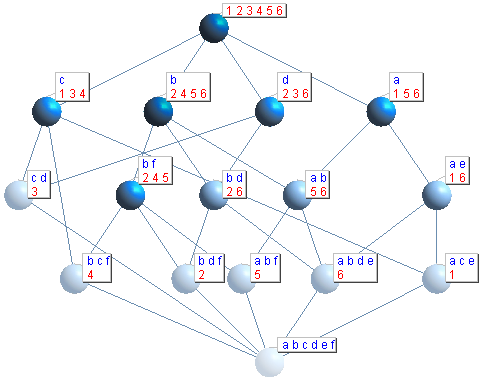
\includegraphics[scale=0.50]{figures/exemple-treillis.png}\end{center}
\caption{Treillis avec étiquetage complet pour le contexte du tableau \ref{cap:context-simple}}
\end{figure}
\end{frame}

%------------------------------------------------
\begin{frame}
\frametitle{Rappels V}
\framesubtitle{Analyse formelle de concepts}
\begin{figure}[H]
\label{cap:fig:treillis-reduced-labelling}
\begin{center}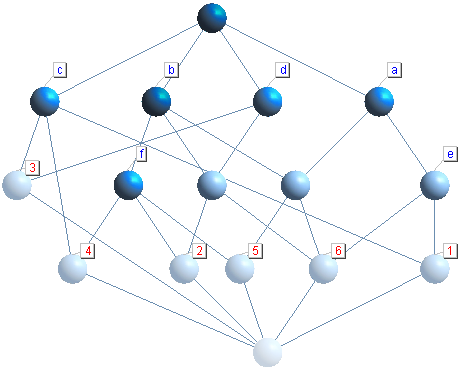
\includegraphics[scale=0.50]{figures/treillis-reduced-labelling.png}\end{center}
\caption{Treillis avec étiquetage réduit pour le contexte du tableau \ref{cap:context-simple}}
\end{figure}
\end{frame}

%------------------------------------------------
\begin{frame}
\frametitle{Rappels VI}
\framesubtitle{Analyse formelle de concepts}
L'\emph{infimum} est le plus petit concept d'un treillis de Galois alors que le \emph{supremum} est son plus grand concept.

Lorsqu'un concept $c_1$ est plus petit qu'un autre concept $c_2$, alors le nœud représentant $c_1$ est placé plus bas que son successeur $c_2$. Lorsqu'une relation d'ordre existe entre les concepts $c_1$ et $c_2$, on dit alors que ces concepts sont \textit{comparables} ($\leq$), sinon ils ne le sont pas ($\not\leq$).
\begin{block}{Définition 6: sup-irréductible et inf-irréductible}
On rappelle qu'un concept est dit \emph{sup-irréductible} (ou \emph{join-irréductible}) si et seulement si il possède un unique prédécesseur et il est dit \emph{inf-irréductible} (ou \emph{meet-irréductible}) s'il admet un unique successeur.
\end{block}
\end{frame}

%------------------------------------------------
\begin{frame}
\frametitle{Rappels VII}
\framesubtitle{Règles d'association et implications}
\begin{block}{Définition 7: règle d'association}
$$r : Y \rightarrow Z\ [sup, conf]$$
$r$ est une règle d'association avec
\begin{itemize}
\item $Y$ et $Z$ sont des sous-ensembles d'attributs appelés \textit{itemsets},
\item $Y \cap Z = \emptyset$,
\item \textit{sup}, le support est $Prob(Y \cup Z)$ (proportion des objets ayant simultanément les attributs $Y$ et $Z$), et
\item \textit{conf}, la confiance est $Prob(Y \cup Z)$ (probabilité d'avoir $Z$ lorsque $Y$ est présent dans le contexte \context).
\end{itemize}
\end{block}
\end{frame}

%------------------------------------------------
\begin{frame}
\frametitle{Rappels VIII}
\framesubtitle{Règles d'association et implications}
\begin{block}{Définitions 8: itemsets et générateurs}
\begin{itemize}
\item Un \emph{itemset} est dit \emph{fréquent} si la proportion d'objets le possédant est au moins égale au support minimum défini par l'utilisateur.
\item Un \emph{itemset} $Y$ est dit \emph{fermé} si $Y = Y''$. Cela signifie que $Y$ est une intention d'un concept formel.
\item Un \emph{générateur} $G$ \parencite{Pfaltz2002} d'un itemset fermé (intention) $Y$ est un ensemble minimal de  $Y$
tel que $G''= Y$. 
\end{itemize}
\end{block}
\end{frame}


%------------------------------------------------
\begin{frame}
\frametitle{Rappels IX}
\framesubtitle{Règles d'association et implications}
\begin{block}{Définition 9: implication et base générique}
$$r: g_i \rightarrow Int(c)\ \backslash\ g_i $$
$r$ est une implication ou règle exacte avec
\begin{itemize}
\item $c$ un concept formel,
\item $G=\{g_1,\ldots g_i, \ldots g_n \}$ l'ensemble de ses générateurs,
\item $Int(c)$ représente l'intention du concept $c$,
\item \emph{support}$(c)$ est la proportion d'objets contenus dans l'extension de $c$,
\item \emph{support}$(r) = $ \emph{support}$(c)$ et
\item \emph{confiance}$(r) = 100\ \%$
\end{itemize}
Une base générique \parencite{Pasquier1999} d'implications est une représentation relativement concise d'implications de la forme précédente. 
\end{block}
\end{frame}

%------------------------------------------------
\begin{frame}
\frametitle{Rappels X}
\framesubtitle{Règles d'association et implications}
\begin{block}{Définition 10: règle approximative}
$$r: g_i \rightarrow Int(c_j)\backslash Int(c) $$
$r$ est une règle approximative avec
\begin{itemize}
\item $c$ un concept formel,
\item $P = \{c_1, \ldots, c_j, \ldots \}$ l'ensemble des prédecesseurs de $c$,
\item $Int(c)$ représente l'intention du concept $c$,
\item $g_i$ un générateur de $Int(c)$,
\item \emph{support}$(r) =$ \emph{support}$(c_j)$, et
\item  \emph{confiance}$(r) = $\emph{support}$(c_j)/support(c)$
\end{itemize}
\end{block}
\end{frame}

%------------------------------------------------
\begin{frame}
\frametitle{Rappels XI}
\framesubtitle{Règles d'association et implications}
\begin{block}{Définitions 11: pseudo-intent et base de Guigues-Duquenne}
Un ensemble $P \subseteq M$ est un \emph{pseudo-intent} de $(G, M, I)$ ~\parencite{Ganter1999,Guigues1986} si et seulement si $P \neq P''$ et si $Q'' \subseteq P$ est vraie pour tout pseudo-intent $Q \subseteq P$, $Q \ne P.$ \\
L'ensemble des implications de la forme :
$$\cal{L} := \{ P \rightarrow P''\ \backslash\ P\ |\ P\ \textit{pseudo-intent}\ \}$$
est appelé base de Guigues-Duquenne (\emph{stem base}) et reconnue comme étant minimale.
\end{block}
À titre d'exemple, $\{a, c\}$ est un pseudo-intent dont le fermé est $\{a, c, e\}$, d'où l'implication $\{a, c\} \rightarrow \{e\}$
\end{frame}

%------------------------------------------------
\begin{frame}
\frametitle{Rappels XII}
\framesubtitle{Règles d'association et implications}
\begin{figure}[H]
\label{cap:fig:treillis-gen}
\begin{center}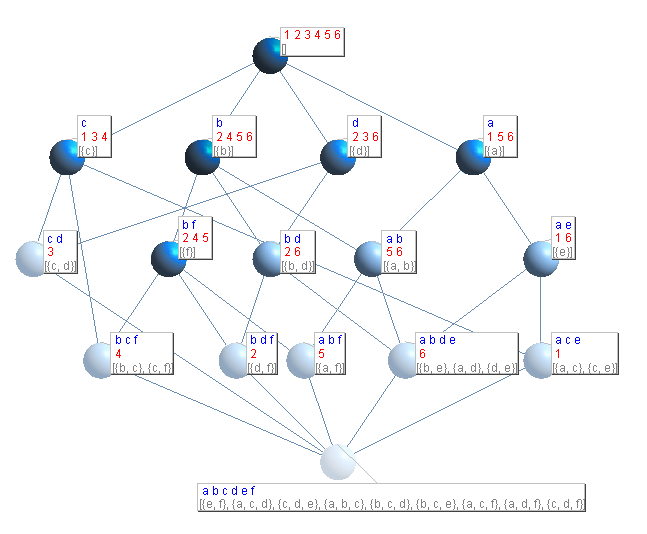
\includegraphics[scale=0.36]{figures/Treillis21FullLabelGen.png}\end{center}
\caption{Treillis de concepts avec indication des générateurs}
\end{figure}
\end{frame}

%------------------------------------------------
\begin{frame}
\frametitle{Rappels XIII}
\framesubtitle{Règles d'association et implications}
\begin{block}{Définition 12: contexte complémentaire  $\KKn$}
Soit un contexte $\KK = \GMI$ décrivant un ensemble $G$ d’objets, un ensemble $M$ de propriétés (attributs) et une relation binaire $I$ entre $G$ et $M$. Le contexte complémentaire de $\KK$ est $\KKn = (G, \tilde{M}, G \times M \backslash I)$ avec $\tilde{M}$ l'ensemble des attributs négatifs.
\end{block}
\begin{block}{Définition 13: apposition du contexte $\KK$ avec son complémentaire $\KKn$}
Le contexte $\KKc$ est l'apposition du contexte $\KK$ avec son complémentaire $\KKn$. Cela signifie que $\KKc:= (G, M \cup \tilde{M}, I \cup G \times M \backslash I)$.
\end{block}
\end{frame}

%------------------------------------------------
\begin{frame}
\frametitle{Rappels XIV}
\framesubtitle{Règles d'association et implications}
\begin{figure}[h]
\label{cap:fig:negctx}
\begin{center}
\begin{cxt}%
\cxtName{}%
\att{a}%
\att{b}%
\att{c}%
\att{d}%
\att{e}%
\att{f}%
\att{$\tilde{a}$}%
\att{$\tilde{b}$}%
\att{$\tilde{c}$}%
\att{$\tilde{d}$}%
\att{$\tilde{e}$}%
\att{$\tilde{f}$}%
\obj{x.x.x..x.x.x}{1}
\obj{.x.x.xx.x.x.}{2}
\obj{..xx..xx..xx}{3}
\obj{.xx..xx..xx.}{4}
\obj{xx...x..xxx.}{5}
\obj{xx.xx...x..x}{6}
\end{cxt}
\end{center}
\caption{$\mathbb{K}|\tilde{\mathbb{K}}$ : apposition du contexte $\KK$ avec son complémentaire $\KKn$}
\end{figure}
\end{frame}

%------------------------------------------------
\begin{frame}
\frametitle{Rappels XV}
\framesubtitle{Relations flèches}
\begin{block}{Définition 14: Relations flèches}
La relation entre l'objet $g$ et l'attribut $m$ dans un contexte formel se présente sous l'une des quatre formes suivantes~:
\begin{itemize}
\item $g \updownarrow m$ si $\gamma(g) \not\leq \mu(m)$, $\gamma(g) \leq m^+$, et $g^- \leq \mu(m)$
\item $g \uparrow m$ si $\gamma(g) \not\leq \mu(m)$, $\gamma(g) \leq m^+$, et $g^- \not\leq \mu(m)$
\item $g \downarrow m$ si $\gamma(g) \not\leq \mu(m)$, $\gamma(g) \not\leq m^+$, et $g^- \leq \mu(m)$
\item $g \circ m$ si $\gamma(g) \not\leq \mu(m)$, $\gamma(g) \not\leq m^+$, et $g^- \not\leq \mu(m)$
\end{itemize}
où $g^-$ représente le prédécesseur immédiat du concept objet (sup-irréductible) $\gamma(g)$ 
et $m^+$ représente le successeur immédiat du concept attribut (inf-irréductible) $ \mu(m)$.
\end{block}
\end{frame}

%------------------------------------------------
\begin{frame}
\frametitle{Rappels XVI}
\framesubtitle{Relations flèches}
\begin{figure}[h]
\label{cap:fig:arrow}
\begin{center}
\begin{cxt}%
\cxtName{}%
\att{a}%
\att{b}%
\att{c}%
\att{d}%
\att{e}%
\att{f}%
\obj{xbxbxd}{1}
\obj{bxbxdx}{2}
\obj{bbxxdd}{3}
\obj{bxxbdx}{4}
\obj{xxbbbx}{5}
\obj{xxbxxb}{6}
\end{cxt}
\end{center}
\caption{Relation flèches pour le contexte $\KK$}
\end{figure}
Par exemple, $3 \downarrow e$ car 
\begin{itemize}
\item $\gamma(3) \not\leq \mu(e)$ avec $\gamma(3)= (3, cd)$ et $\mu(e)=(16, ae)$
\item $\gamma(3) \not\leq e^+$ avec $e^+ = (156,a)$
\item $3^- \leq \mu(e)$ avec $3^-=(\emptyset, abcdef)$
\end{itemize}
\end{frame}

%------------------------------------------------
\section{Les outils de l'analyse formelle de concepts}
%------------------------------------------------
\begin{frame}
\huge{\centerline{Les outils de l'analyse formelle de concepts}}
\end{frame}
%------------------------------------------------
\begin{frame}
\frametitle{Les outils de l'analyse formelle de concepts}
\framesubtitle{\textsc{Galicia}}
\begin{itemize}
\item \textsc{Galicia}\footnote{\url{http://www.iro.umontreal.ca/~galicia/}} a été developpé en Java par Pekto Valchev et ses collaborateurs (Université de Montréal).
\end{itemize}
\begin{columns}[c] % The "c" option specifies centered vertical alignment while the "t" option is used for top vertical alignment

\column{.45\textwidth} % Left column and width
\begin{figure}[H]
\begin{center}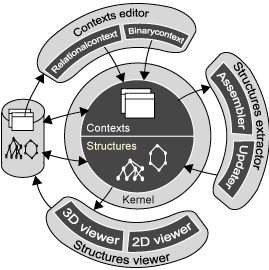
\includegraphics[scale=0.40]{figures/galicia-life-cycle.png}\end{center}
\caption{Cycle de vie du treillis Galicia}
\label{cap:fig:galicia-life-cycle}
\end{figure}

\column{.5\textwidth} % Right column and width
Quelques fonctionnalités de Galicia:
\begin{itemize}
\item Affichage du treillis en trois dimensions
\item Manipulation du contexte et du treillis
\item Plusieurs procédures de construction du treillis : Bordat, Nourine, Godin et \emph{Next-Closure}
\item Connection à des bases de données SQL pour sauvegarder les contextes
\end{itemize}
\end{columns}

\end{frame}
%------------------------------------------------
\begin{frame}
\frametitle{Les outils de l'analyse formelle de concepts}
\framesubtitle{\textsc{Galicia}}
\begin{columns}[c] % The "c" option specifies centered vertical alignment while the "t" option is used for top vertical alignment
\column{.4\textwidth} % Left column and width
\begin{figure}[H]
\label{fig:galicia-ctx}
\begin{center}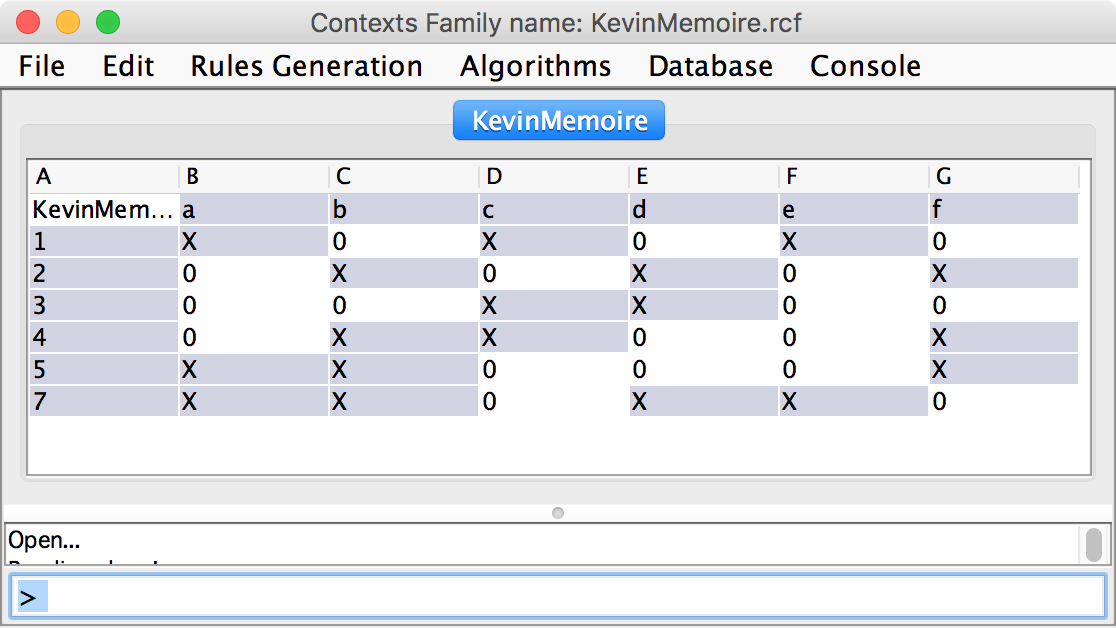
\includegraphics[scale=0.28]{figures/galicia1.jpg}\end{center}
\caption{Éditeur de contexte}
\end{figure}
\column{.6\textwidth} % Right column and width
\begin{figure}[H]
\begin{center}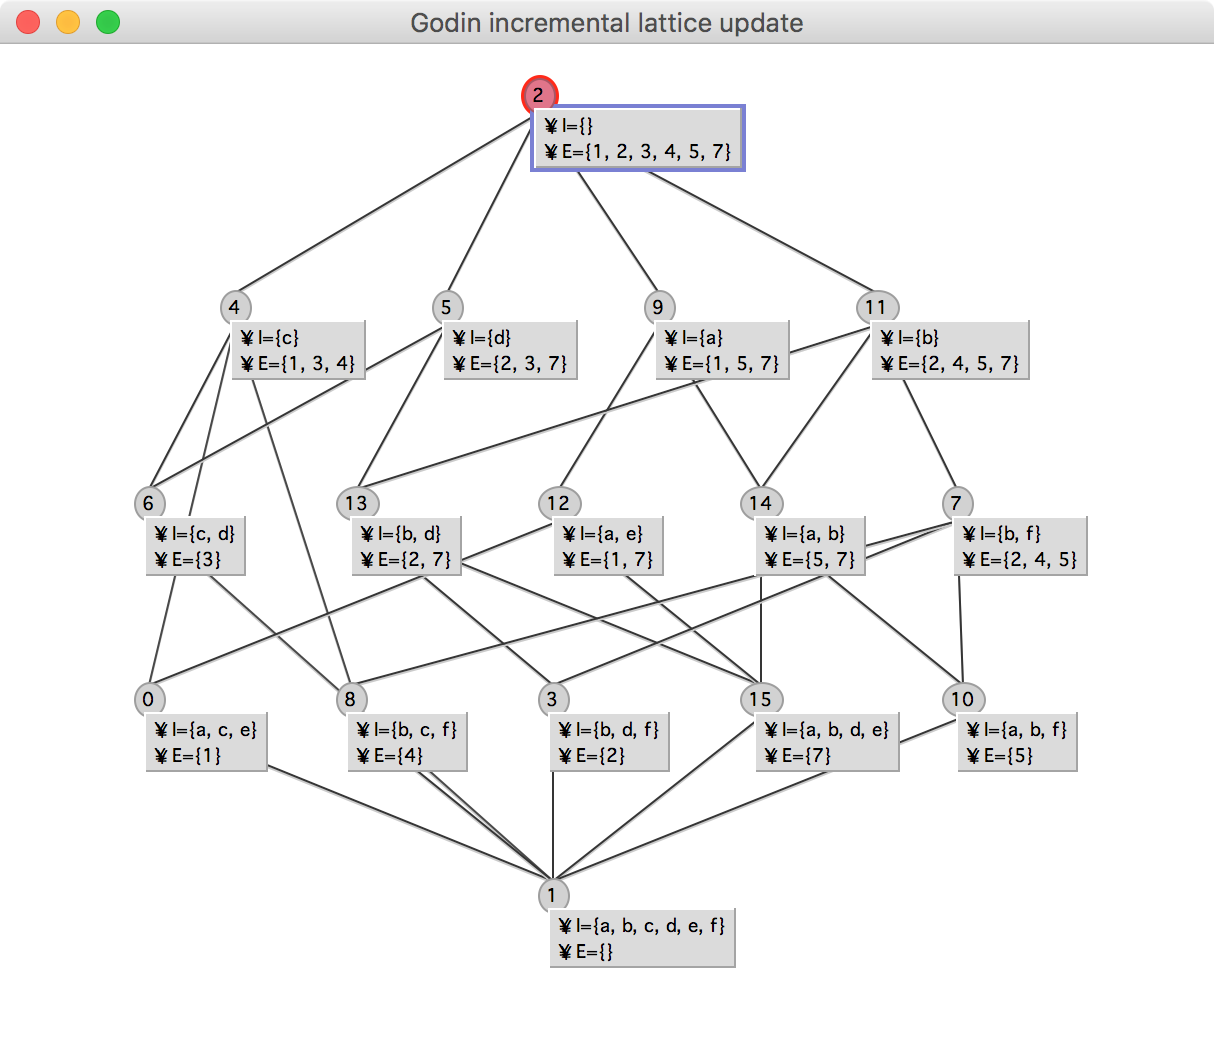
\includegraphics[scale=0.30]{figures/galicia-full-labeling.png}\end{center}
\caption{Treillis Galicia avec étiquetage complet}
\label{cap:fig:galicia-full-label}
\end{figure}
\end{columns}
\end{frame}
%------------------------------------------------
\begin{frame}
\frametitle{Les outils de l'analyse formelle de concepts}
\framesubtitle{Le système Coron}
Le système Coron\footnote{\url{http://coron.loria.fr/site/index.php}.}~\parencite{Szathmary2006} est une boîte à outils qui a été développée au laboratoire LORIA\footnote{Laboratoire lorrain de recherche en informatique et ses applications, Nancy, France} 
\begin{columns}[t]
\column{.45\textwidth} % Left column and width
\begin{itemize}
\item Développé avec Java et Perl
\item En ligne de commandes
\item Version actuelle de ce système est 0.8 et date de janvier 2010
\item Compatible avec les systèmes d'exploitation Unix, macOS et Windows
\end{itemize}
\column{.55\textwidth} % Right column and width
\begin{itemize}
\item Implémente plusieurs algorithmes de fouille de données tels qu'Apriori, Close, Aclose, Carpathia, Charm, Next-Closure ou NFI-Simple.
\item Simple d'utilisation, modulaire et documentation riche
\item Code source non disponible
\end{itemize}
\end{columns}
\end{frame}
%------------------------------------------------
\begin{frame}
\frametitle{Les outils de l'analyse formelle de concepts}
\framesubtitle{Librairie Java Lattices}
La libraire \textit{Java Lattices}\footnote{\url{https://thegalactic.github.io/java-lattices}}~\parencite{Bertet2014} a été développée par le laboratoire L3i\footnote{Laboratoire Informatique, Image et Interaction, université de La Rochelle, France}.
\begin{columns}[t]
\column{.45\textwidth} % Left column and width
\begin{itemize}
\item Permet de générer des treillis de Galois et des règles d'association
\item Code source libre et disponible sur la plate-forme GitHub
\item Entièrement écrit avec Java
\end{itemize}
\column{.55\textwidth} % Right column and width
\begin{itemize}
\item La libraire est compatible avec Maven (outil Java pour gérer les dépendances)
\item Client en ligne de commandes disponible
\item Algorithme \emph{Limited Object Access (LOA)}~\parencite{Demko2011}
\end{itemize}
\end{columns}
\end{frame}
%------------------------------------------------
\begin{frame}
\frametitle{Les outils de l'analyse formelle de concepts}
\framesubtitle{ToscanaJ}
\emph{ToscanaJ}~\parencite{Becker2002} est une réimplémentation avec le langage de programmation Java de l'outil d'AFC connu sous le nom de <<~\emph{Toscana}~>>. Cet outil a la particularité d'être le premier outil à offrir l'affichage des diagrammes imbriqués (\emph{nested line diagrams}) comme on peut le voir avec la figure~\ref{cap:fig:toscanaj-nested}.
\begin{figure}[H]
\caption{ToscanaJ: Diagrammes imbriqués}
\label{cap:fig:toscanaj-nested}
\begin{center}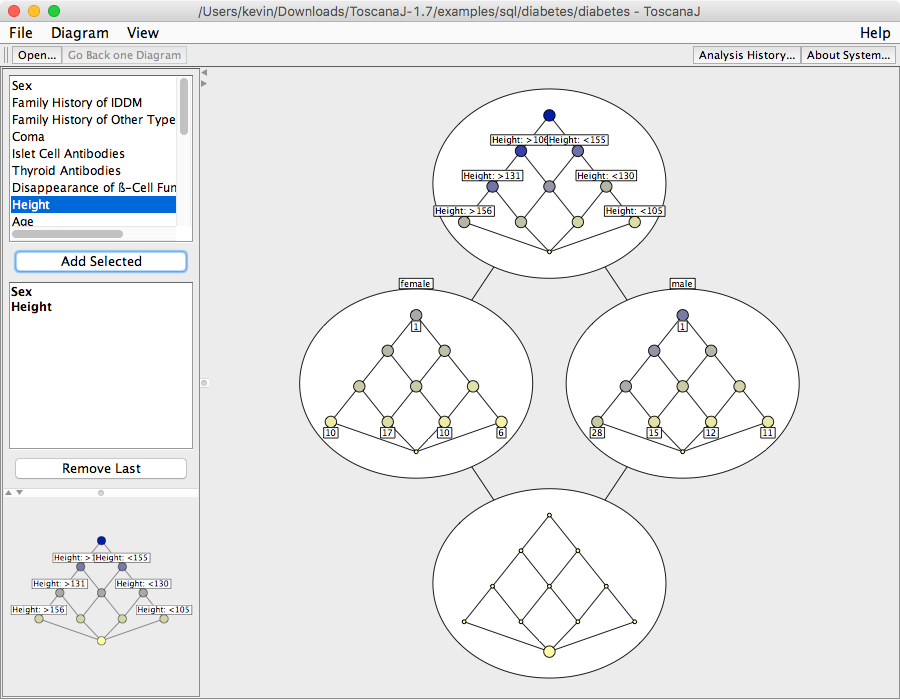
\includegraphics[scale=0.17]{figures/toscanaj-nested.png}\end{center}
\end{figure}
\end{frame}
%------------------------------------------------
\begin{frame}
\frametitle{Les outils de l'analyse formelle de concepts}
\framesubtitle{Concept Explorer}
\emph{Concept Explorer}\footnote{\url{http://conexp.sourceforge.net/}} (\emph{ConExp}) est un outil souvent utilisé par les chercheurs en AFC.
\begin{itemize}
\item Interface graphique complète en Java Swing
\item Édition et transformation de contextes
\item Construction de treillis de concepts
\item Code distribué librement
\item Base Guigues-Duquenne
\item Génération des règles d'association et l'exploration des attributs
\item Génération des relations flèches
\end{itemize}
Dans le cadre de ce mémoire, nous allons utiliser \emph{ConExp} à des fins de validation, notamment pour tester la procédure de production des relations flèches et pour la génération de la base de Guigues--Duquenne.

\end{frame}
%------------------------------------------------
\begin{frame}
\frametitle{Les outils de l'analyse formelle de concepts}
\framesubtitle{Concept Explorer}
\begin{columns}[c]
\column{.4\textwidth} % Left column and width
\begin{figure}[H]
\label{cap:fig:conexp-associations}
\begin{center}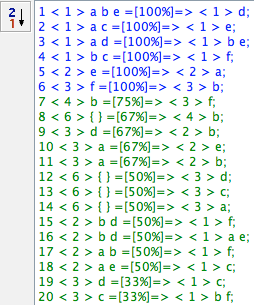
\includegraphics[scale=0.45]{figures/conexp-associations.png}\end{center}
\caption{\emph{ConExp}: Règles d'association}
\end{figure}
\column{.6\textwidth}
\color{green!40!teal}
\texttt{7 < 4 > b =[75\%]=> < 3 > f;} \\
\color{black}
Il s'agit de la 7-ème règle d'association laquelle indique que $b$ implique $f$ avec un support absolu de 3 parmi les six objets (et donc un support relatif de $50 \%$) et une confiance de $75 \%$.
\end{columns}
\end{frame}
%------------------------------------------------
\begin{frame}
\frametitle{Les outils de l'analyse formelle de concepts}
\framesubtitle{Concept Explorer}
\begin{figure}[H]
\begin{center}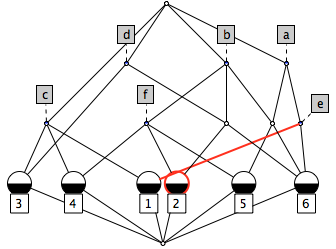
\includegraphics[scale=0.45]{figures/conexp-lattice.png}\end{center}
\caption{\emph{ConExp}: Affichage du treillis}
\label{cap:fig:conexp-lattice}
\end{figure}
\begin{itemize}
\item L'affichage du treillis se fait selon un étiquetage réduit seulement.
\item \emph{ConExp} utilise un algorithme de construction du treillis avec le minimum d'intersections et les collisions sont affichées en rouge.
\end{itemize}
\end{frame}
%------------------------------------------------
\begin{frame}
\frametitle{Les outils de l'analyse formelle de concepts}
\framesubtitle{\lm}
\begin{itemize}
\item Logiciel en Java pour la visualisation et la manipulation de treillis
\item Intialement conçu par Geneviève Roberge dans le cadre de son mémoire de maîtrise.
\item Continuellement enrichi par les membres de l'équipe et plusieurs stagiaires ingénieurs français.
\item Aussi bien dans sa version initiale que dans sa version révisé, \lm est un logiciel libre disponible sur \emph{SourceForge}\footnote{\url{https://sourceforge.net/projects/lattice-miner/}} et GitHub\footnote{\url{https://github.com/LarimUQO/lattice-miner}}.
\end{itemize}
\end{frame}
%------------------------------------------------
\begin{frame}
\frametitle{Les outils de l'analyse formelle de concepts}
\framesubtitle{\lm}
\begin{figure}[H]
\caption{Génération du treillis de concepts dans \lm}
\label{cap:fig:lm-treillis}
\begin{center}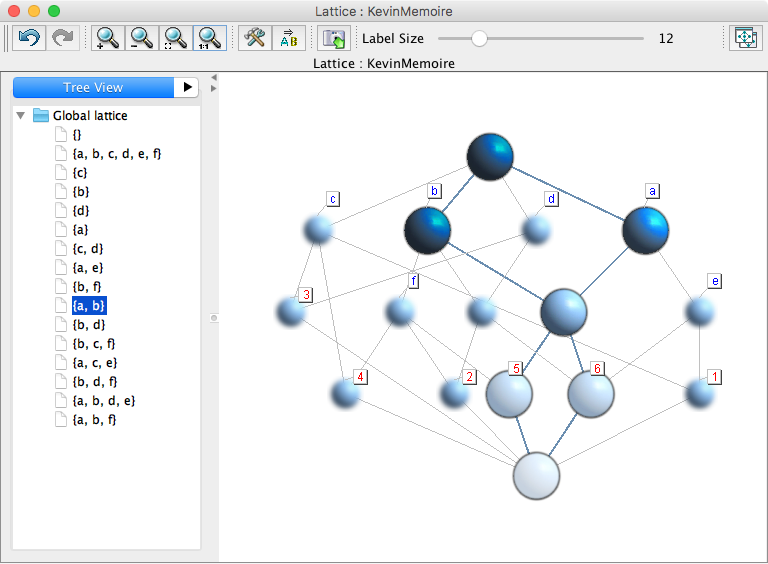
\includegraphics[scale=0.32]{figures/lm-treillis.jpg}\end{center}
\end{figure}
\end{frame}
%------------------------------------------------
\begin{frame}
\frametitle{Les outils de l'analyse formelle de concepts}
\framesubtitle{\lm}
\begin{figure}[H]
\caption{Approximation dans \lm}
\label{cap:fig:lm-approxime}
\begin{center}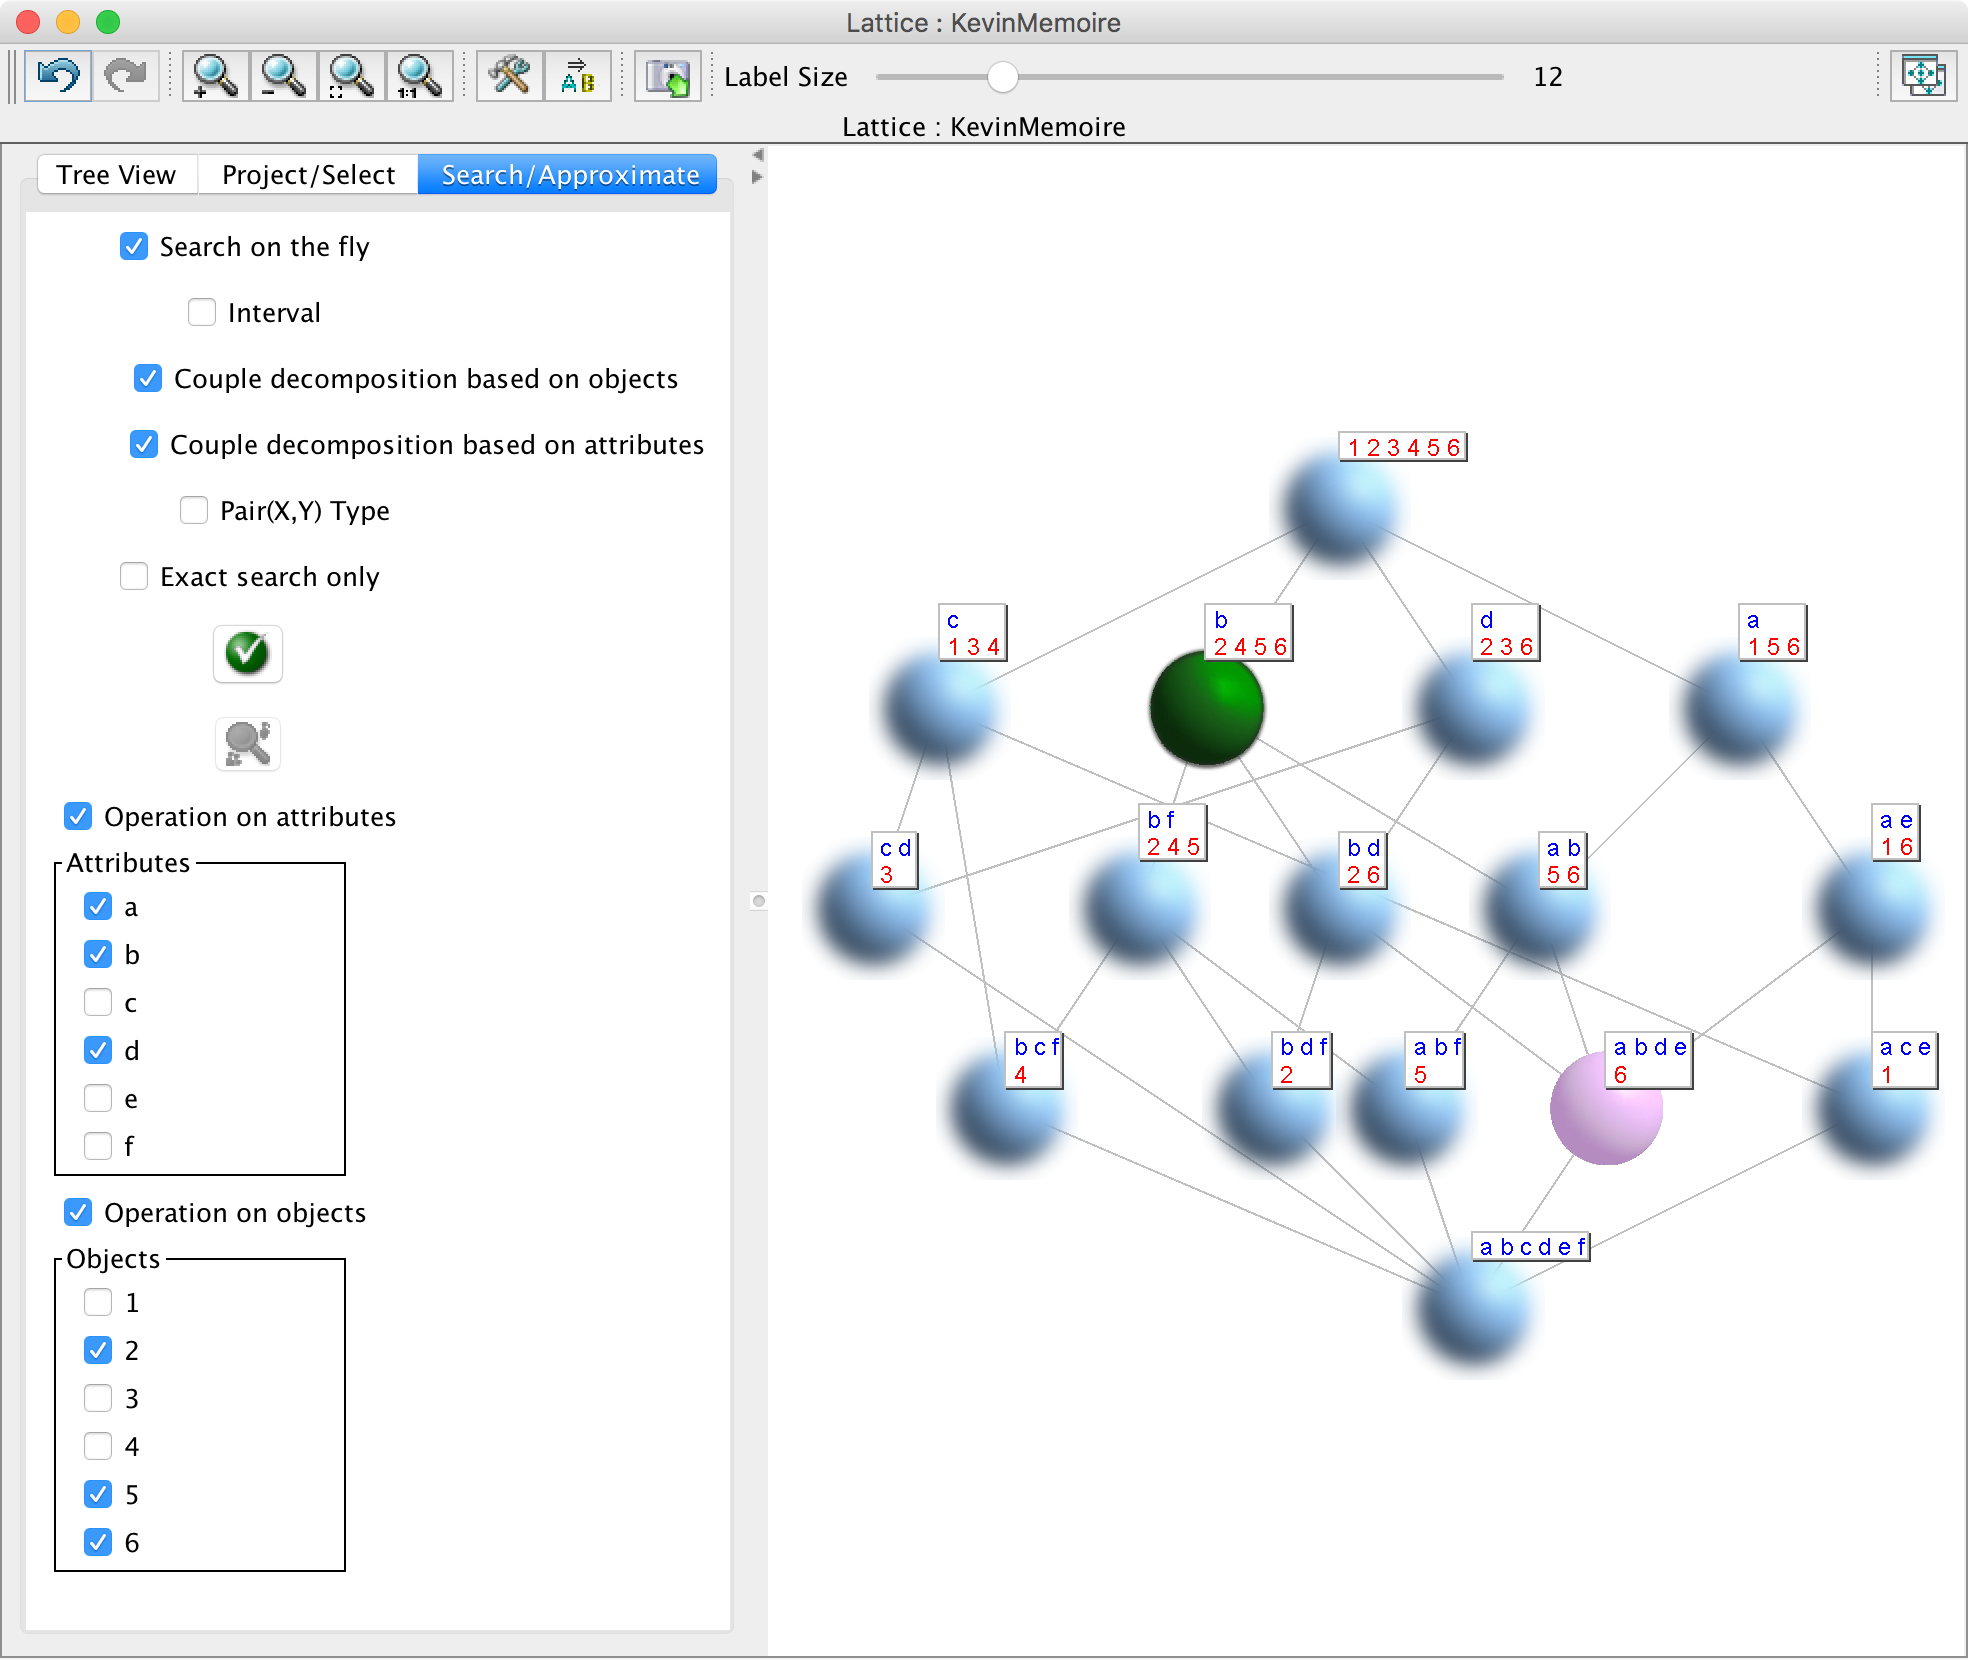
\includegraphics[scale=0.22]{figures/Approxime.PNG}\end{center}
\end{figure}
\end{frame}
%------------------------------------------------
\begin{frame}
\frametitle{Les outils de l'analyse formelle de concepts}
\framesubtitle{\lm}
\begin{figure}[H]
\caption{Affichage de l'apposition d'un contexte avec son complémentaire}
\label{cap:fig:lm-complem-ctx}
\begin{center}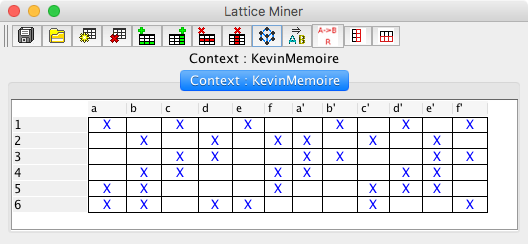
\includegraphics[scale=0.45]{figures/lm-complem-ctx.jpg}\end{center}
\end{figure}
\end{frame}
%------------------------------------------------
\begin{frame}
\frametitle{Les outils de l'analyse formelle de concepts}
\framesubtitle{\lm}
\begin{figure}[H]
\caption{Base générique d'implications avec possibilité de redondance}
\label{cap:fig:Imp-Red}
\begin{center}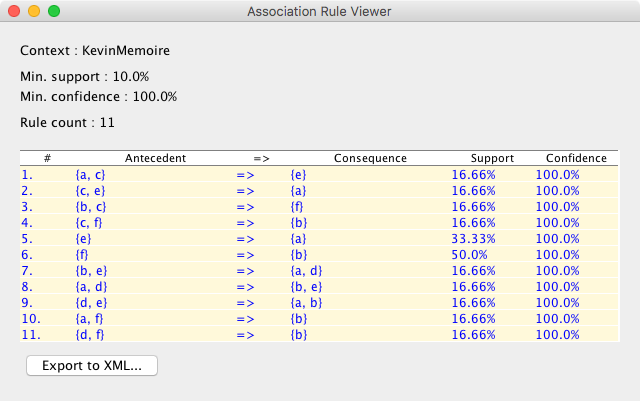
\includegraphics[scale=0.45]{figures/ImplRed.png}\end{center}
\end{figure}
\end{frame}
%------------------------------------------------
\begin{frame}
\frametitle{Les outils de l'analyse formelle de concepts}
\framesubtitle{\lm}
\begin{figure}[H]
\caption{Base générique d'implications sans redondance}
\label{cap:fig:Imp-NonRed}
\begin{center}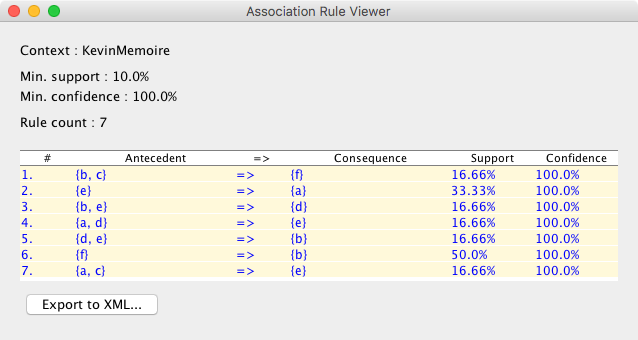
\includegraphics[scale=0.45]{figures/ImplNonRed.png}\end{center}
\end{figure}
\end{frame}
%------------------------------------------------
\begin{frame}
\frametitle{Les outils de l'analyse formelle de concepts}
\framesubtitle{\lm}
\begin{figure}[H]
\caption{Relations flèches dans \lm}
\label{cap:fig:lm-arrows}
\begin{center}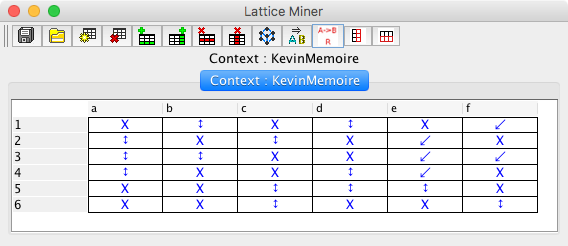
\includegraphics[scale=0.45]{figures/lm-arrow.jpg}\end{center}
\end{figure}
\end{frame}

%------------------------------------------------
\section{Production d'implications avec négation}
%------------------------------------------------
\begin{frame}
\huge{\centerline{Production d'implications avec négation}}
\end{frame}
%------------------------------------------------

%------------------------------------------------
\begin{frame}[allowframebreaks]
\frametitle{References}
\printbibliography
\end{frame}
%------------------------------------------------
\begin{frame}
\Huge{\centerline{Questions ?}}
\end{frame}
%------------------------------------------------

\end{document} 